\documentclass{article}

\usepackage[left=1in, top=1in, right=1in, bottom=1in]{geometry}
\usepackage{graphicx, color}
\usepackage{amsmath}
\usepackage{amsthm}
\usepackage{amssymb}
\usepackage{url}
\usepackage{apacite}
\usepackage{float}
\usepackage[linesnumbered,ruled,vlined]{algorithm2e}
\usepackage{framed}
\usepackage{here}
\usepackage{zi4}
\usepackage{color}
\usepackage{Sweave}

\DeclareMathOperator*{\argmin}{arg\,min}
\DeclareMathOperator*{\argmax}{arg\,max}
\DeclareMathOperator*{\median}{median}


\renewcommand{\baselinestretch}{1.2}

% \VignetteIndexEntry{glmnetLRC Example}

\begin{document} 
\Sconcordance{concordance:glmnetLRC.tex:/Users/d3p423/Work/github/glmnetLRC/vignettes/glmnetLRC.Rnw:%
1 54 1 1 3 2 0 1 3 1 0 1 3 14 0 1 4 5 0 1 2 7 1 1 4 3 0 1 2 6 0 1 2 4 1 %
1 5 4 0 1 3 9 0 1 2 16 1 1 3 2 0 1 6 8 0 1 3 6 1 1 2 9 0 1 2 3 1 1 2 12 %
0 1 2 12 1 1 3 2 0 1 4 14 0 1 2 4 1 1 3 13 0 1 2 1 3 2 0 1 3 8 0 1 3 1 %
0 1 3 12 0 1 3 12 0 1 2 1 1 1 2 9 0 1 2 13 1 1 2 5 0 1 2 176 1}


\title{{\tt glmnetLRC}: Lasso and elastic-net logistic regression classification with an arbitrary loss function\\}
\author{Landon Sego, Alexander Venzin}
\maketitle

\section{Introduction}

The {\tt glmnetLRC} package makes it easy to create a binary classifier that uses virtually any number of quantitative predictors to
assign an example, or observation, to one of two classes.
It extends the {\tt glmnet} package by making it possible to train lasso or elastic-net logistic 
regression classifiers (LRC's) using a customized, discrete loss function to measure the classification error.  
This allows users to assign unique 
loss values to false positive and false negative errors. The logistic regression parameter
estimates are obtained by maximizing the elastic-net penalized likelihood function that contains several tuning parameters. These
tuning parameters are estimated by minimizing the expected loss, which is calculated using cross validation.
This approach was originally implemented to automate the
process of determining the curation quality of mass spectrometry samples \cite{Amidan}. Those same data
will be used here to demonstrate how to train your own classifier.

In the sections that follow, we show how to use the {\tt glmnetLRC} package to train LRC models, create diagnostic plots,
extract coefficients, predict the binary class of new observations, and summarize the performance of those
predictions. The details of the algorithms used by the package are provided in final section of the document.

\section{Training}

Let's begin by loading the package and the training data:
\begin{Schunk}
\begin{Sinput}
> # Load the package
> library(glmnetLRC)
> # Load the VOrbitrap Shewanella QC data
> data(traindata)
> # A view of first two rows and first 12 columns
> traindata[1:2, 1:12]
\end{Sinput}
\begin{Soutput}
      Instrument_Category Instrument Dataset_ID Acq_Time_Start Acq_Length
pt701           VOrbitrap VOrbiETD03     251690     12/31/2011         98
pt702           VOrbitrap VOrbiETD03     251706       1/1/2012         98
                                          Dataset Dataset_Type Curated_Quality
pt701 QC_Shew_11_06_col2A_30Dec11_Cougar_11-10-11      HMS-MSn            good
pt702 QC_Shew_11_06_col2C_30Dec11_Cougar_11-10-11      HMS-MSn            good
      XIC_WideFrac XIC_FWHM_Q1 XIC_FWHM_Q2 XIC_FWHM_Q3
pt701     0.297090     19.3820     21.1900     24.3149
pt702     0.305519     19.3785     21.1812     24.3262
\end{Soutput}
\begin{Sinput}
> # Columns 9 to 96 contain various measures of dataset quality that
> # we will use to predict the "Curated_Quality"
> predictors <- as.matrix(traindata[,9:96])
\end{Sinput}
\end{Schunk}

\noindent We fit the LRC model by calling {\tt glmnetLRC()}, which 
requires a binary response variable, coded
as a {\tt factor}.  The order in which the response variable
is coded is important.  Specifically, the class we want to predict with
the greatest sensitivity should be encoded as the second level. To illustrate how this
is done, consider the Shewanella QC data, where the objective is to be
sensitive to predicting poor datasets.  Hence we code ``poor" last, as follows:
\begin{Schunk}
\begin{Sinput}
> response <- factor(traindata$Curated_Quality,
+                    levels = c("good", "poor"),
+                    labels = c("good", "poor"))
> levels(response)
\end{Sinput}
\begin{Soutput}
[1] "good" "poor"
\end{Soutput}
\end{Schunk}
\noindent Now we must define a discrete loss matrix. For the curation
of dataset quality, predicting ``good" when the dataset is ``poor" is considerably 
worse (Loss = 5) than predicting ``poor" when the dataset
is ``good" (Loss = 1).  Correct predictions receive a penalty of zero loss:

\begin{Schunk}
\begin{Sinput}
> # Define the loss matrix
> lM <- lossMatrix(c("good","good","poor","poor"),
+                  c("good","poor","good","poor"),
+                  c(     0,     1,     5,     0))
> # Observe the structure of the loss matrix
> lM
\end{Sinput}
\begin{Soutput}
           Predicted.good Predicted.poor
Truth.good              0              1
Truth.poor              5              0
\end{Soutput}
\end{Schunk}

To train an elastic-net model, the user needs to supply a handful of arguments to {\tt glmnetLRC()}. 
The mandatory arguments are the true class labels, {\tt truthLabels} (which, in this case, is, is the {\tt response} 
object we created above), the matrix of predictor variables, {\tt predictors}, 
and the loss matrix {\tt lossMat}. Noteworthy additional arguments include {\tt tauVec}, a vector of potential values of the 
threshold parameter $\tau \in (0, 1)$ that are used to dichotomize the predicted probabilities from the logistic regression 
into two class labels; {\tt alphaVec}, a vector of potential values of the elastic-net mixing parameter 
$\alpha \in [0, 1]$; {\tt cvFolds}, the number of cross validation folds; {\tt cvReps}, the number of times
the cross validation process is repeated with a different random partition of the data, and {\tt masterSeed}, which controls 
the partitioning of the data into the cross validation folds. Keep in mind that $\alpha$ governs the tradeoff between 
the two regularization penalties. When $\alpha = 0$, $L_2$ regularization (the ridge penalty) is used,
and when $\alpha = 1$, $L_1$ regularization (the lasso penality) is used.

Heavier sampling of {\tt tauVec} or {\tt alphaVec} (i.e., sequences of greater length) leads to 
increased computation time, but more of the parameter space will be sampled, potentially leading to a better 
classifier.  We now train the elastic-net logistic regression using restricted values of {\tt tauVec} and 
{\tt alphaVec} and a small number of cross validation replicates, {\tt cvReps}.
\begin{Schunk}
\begin{Sinput}
> # Set the number of cores to be one less than the total available
> ncores <- max(1, parallel::detectCores() - 1)
> # Fit the LRC model with 2 cross validation replicates per core
> lrc_fit <- glmnetLRC(response, predictors, lM, nJobs = ncores,
+                      cvFolds = 5, cvReps = 2 * ncores,
+                      alphaVec = c(1, 0.5), tauVec = c(0.3, 0.5, 0.7),
+                      estimateLoss = TRUE)
> 
\end{Sinput}
\end{Schunk}

\noindent The call to {\tt glmnetLRC()} uses cross validation to solve for the optimal parameter settings 
$\left(\alpha, \lambda, \tau\right)$ that minimize the expected loss for the elastic-net logistic regression 
classifier. Printing the resulting object shows the median value for the parameters over the cross validation 
replicates, as well as the average and standard deviation of the expected loss values calculated for each
cross validation replicate.
 
\begin{Schunk}
\begin{Sinput}
> print(lrc_fit)
\end{Sinput}
\begin{Soutput}
The optimal parameter values for the elastic-net logistic regression fit: 
     Df      %Dev alpha     lambda tau mean.ExpectedLoss sd.ExpectedLoss
[1,]  8 0.6784573     1 0.02983395 0.3         0.1805128      0.01240983
\end{Soutput}
\end{Schunk}

\noindent We can also extract the non-zero coefficients of the elastic-net logistic regression 
model that was created using the optimal values of $\alpha$ and $\lambda$ (which were shown by 
the call to the {\tt print()} method above):
\begin{Schunk}
\begin{Sinput}
> coef(lrc_fit)
\end{Sinput}
\begin{Soutput}
   (Intercept)   XIC_WideFrac  XIC_Height_Q3     MS1_TIC_Q4      MS2_Count 
  6.736524e+00  -1.833107e+01   1.168220e+00   2.556815e-02  -3.431711e-05 
MS2_Density_Q1           C_4A         MS2_4A           P_2B 
 -6.389503e-04   4.202109e-02  -2.422953e-01  -6.532740e-04 
\end{Soutput}
\end{Schunk}

\section{Prediction}

Now that the classifier has been properly trained and the optimal parameters have been identified, we are 
interested in making predictions for new data observations. This requires the elastic-net regression model 
(the output from {\tt glmnetLRC}) and the set of new observations to be predicted, {\tt newdata}.  
Note that {\tt newdata} must contain all the columns (with equivalent names) that were used to train the LRC.
If true labels are available in {\tt newdata}, the column containing 
these true class labels can be specified via the 
{\tt truthCol} argument. Additionally, one may wish to carry through a subset of the explanatory variables in 
{\tt newdata}.  These columns are indicated using {\tt keepCols}.   True labels are not required to make 
predictions---but they are required to compute performance metrics (sensitivity, specificity, etc.) for the 
elastic-net logistic regression model. We begin by testing the classifer on the original training data:
\begin{Schunk}
\begin{Sinput}
> # Predict the training data
> predictTrain <- predict(lrc_fit, traindata, truthCol = "Curated_Quality", keepCols = 1:2)
> # Look at beginning of the predicted data.  Note the extra columns that were 
> # kept:  "Instrument_Category" and "Instrument"
> head(predictTrain)
\end{Sinput}
\begin{Soutput}
      PredictClass Curated_Quality Instrument_Category Instrument
pt701         good            good           VOrbitrap VOrbiETD03
pt702         good            good           VOrbitrap VOrbiETD03
pt703         good            good           VOrbitrap VOrbiETD03
pt704         poor            good           VOrbitrap VOrbiETD03
pt706         poor            poor           VOrbitrap VOrbiETD02
pt707         poor            poor           VOrbitrap VOrbiETD02
\end{Soutput}
\end{Schunk}
\noindent We can summarize the performance of the classifier predictions with a call to the {\tt summary()} method.
The performance metrics are oriented in terms of being sensitive to predicting a ``poor'' dataset.  Thus, a 
false positive is predicting a dataset to be ``poor'' when it is ``good,'' and a false negative is predicting a 
dataset to be ``good'' when it is ``poor.''  This orientation resulted from us setting ``poor'' as the second
level in {\tt response}.
\begin{Schunk}
\begin{Sinput}
> # Summarize the peformance of the new classifier in terms of a variety of metrics:
> summary(predictTrain)
\end{Sinput}
\begin{Soutput}
                          poor
sensitivity         0.91919192
specificity         0.93805310
false negative rate 0.08080808
false positive rate 0.06194690
accuracy            0.93230769
\end{Soutput}
\end{Schunk}
\noindent Now let's bring in some new data and examine the performance of the classifier:
\begin{Schunk}
\begin{Sinput}
> # Load the data for testing
> data(testdata)
> # Create table observing the true number of good/poor items 
> with(testdata, table(Curated_Quality))
\end{Sinput}
\begin{Soutput}
Curated_Quality
good poor 
  38   61 
\end{Soutput}
\begin{Sinput}
> # Predict new data
> predictTest <- predict(lrc_fit, testdata, truthCol = "Curated_Quality")
> # Look at the first few rows
> head(predictTest)
\end{Sinput}
\begin{Soutput}
     PredictClass Curated_Quality
931          poor            good
1449         good            good
1467         good            good
1468         good            good
1470         good            good
1501         good            good
\end{Soutput}
\begin{Sinput}
> # Summarize the output of predicting the test data
> summary(predictTest)
\end{Sinput}
\begin{Soutput}
                          poor
sensitivity         0.90163934
specificity         0.89473684
false negative rate 0.09836066
false positive rate 0.10526316
accuracy            0.89898990
\end{Soutput}
\end{Schunk}
\noindent If we don't include a truth column in the call to {\tt predict()}, the {\tt summary()} method 
counts the number of observations classified to each category:
\begin{Schunk}
\begin{Sinput}
> summary(predict(lrc_fit, testdata))
\end{Sinput}
\begin{Soutput}
 PredictClass
 good:40     
 poor:59     
\end{Soutput}
\end{Schunk}


\section{Diagnostics}

\noindent Finally, we would like to get a sense of the distribution of the tuning parameters that were chosen 
during the cross validation phase. The {\tt plot()} method produces a $3 \times 3$ scatterplot matrix of the optimal 
triples $\left(\alpha, \lambda, \tau\right)$ associated with the selected regression model from each cross 
validation replicate. The univariate distribution of each parameter is plotted on the diagonal of the 
scatterplot matrix.  Ideally, the distributions of the parameters will be tight over the cross validation 
replicates, indicating that the choice of $\left(\alpha, \lambda, \tau\right)$ is stable regardless of
the particular random partition used for cross validation.

\begin{figure}[H]
\begin{center}
\begin{Schunk}
\begin{Sinput}
> plot(lrc_fit)
\end{Sinput}
\end{Schunk}
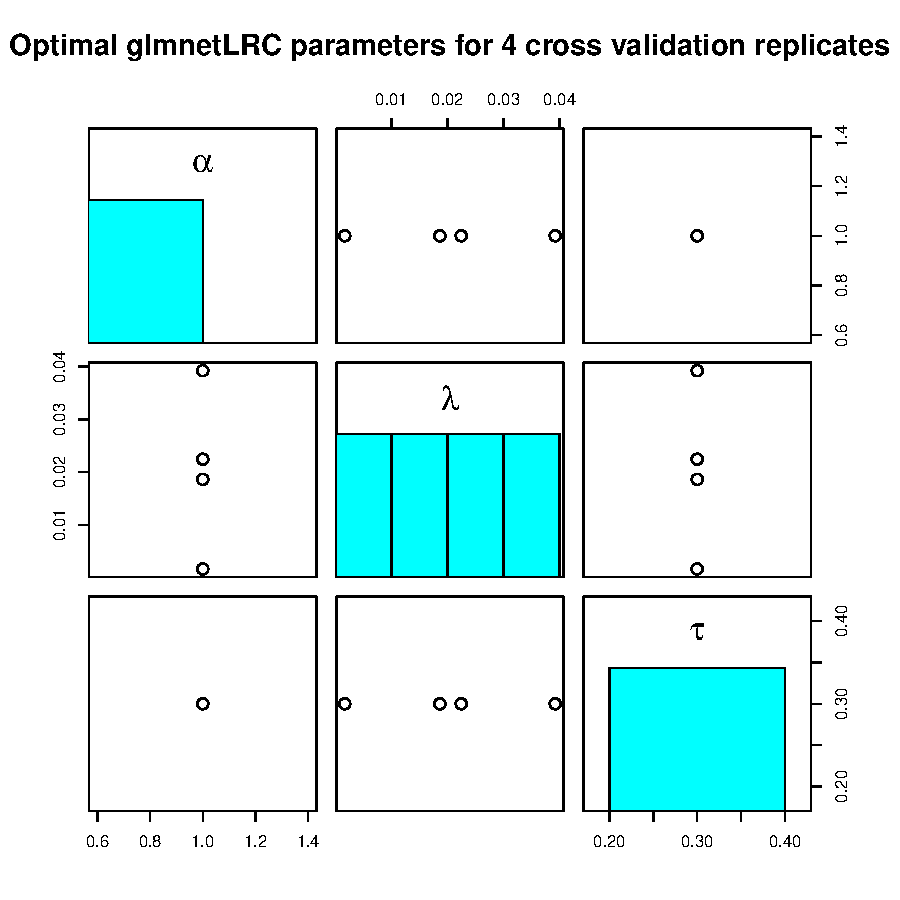
\includegraphics{glmnetLRC-plot}
\caption{Scatterplot matrix of optimal tuning parameters.  Each point represents the optimal estimate of $(\alpha,\lambda,\tau)$
for a given cross validation replicate.}
\end{center}
\end{figure}

\section{Mathematical Details}
We present in detail the algorithm used by the {\tt glmnetLRC} package to identify the optimal parameter estimates
for a logistic regression classifier (LRC) with variables selection implemented by an elastic-net.  

\subsection{The model}

We begin by defining a
number of variables.  Let $i = 1,\ldots,N$ index the observations in a training dataset. 
Let $y_i = 1$ indicate that observation $i$ belongs to category ``1" and $y_i = 0$ indicate
that it belongs to category ``0".  Per the logistic regression model, let  
\begin{align}
%P(y_i = 1) \equiv \pi_i = \pi(\mathbf{x}_i, \boldsymbol{\beta}) = 
P(y_i = 1) \equiv \pi_i = 
\frac{\exp(\beta_0 + \boldsymbol{\beta}_1^T \mathbf{x}_i)}{1+\exp(\beta_0 + \boldsymbol{\beta}_1^T \mathbf{x}_i)}
\end{align}
\noindent where $\mathbf{x}_i = (x_1, \ldots x_p)^T$ is a vector of predictors, or covariates, that
influence $\pi_i$, $\beta_0$ is an intercept, $\boldsymbol{\beta}_1 = (\beta_1, \ldots, \beta_p)^T$ is a 
vector of logistic regression coefficients, and for notational convenience, 
$\boldsymbol{\beta} = (\beta_0, \beta_1, \ldots \beta_p)^T$. 

The estimate of the vector of regression parameters, $\boldsymbol{\beta}$, is influenced by two other tuning parameters, 
$\alpha$ and $\lambda$.  For this reason, we will often write $\boldsymbol\beta$ as $\boldsymbol\beta(\alpha,\lambda)$.  
The value of $\lambda > 0$ controls the weight of the
penalty of the log-likelihoood function, while $\alpha$ controls the mixture of the ridge and lasso penalties.  
The relationship between $\boldsymbol{\beta}$, $\alpha$, and $\lambda$ will be clarified below.  A final tuning parameter, 
$\tau \in (0, 1)$, provides a threshold for the LRC such that if $\pi_i > \tau$, observation $i$ is predicted to belong
to class ``1''.

\subsection{Estimating the regression parameters}

When we fit the elastic-net logistic regression model to the data, we obtain the estimator 
$\hat{\boldsymbol\beta}(\alpha,\lambda)$.  Therefore, 
let $\hat\pi_i \equiv \pi \bigl( \mathbf{x}_i,\hat{\boldsymbol\beta}(\alpha,\lambda) \bigr)$ denote the predicted probability 
that $y_i = 1$.  Then, if $\hat\pi_i > \tau$, the LRC predicts that $y_i = 1$, otherwise it predicts that $y_i = 0$.  
It will be useful to represent the predicted class of observation
$i$ as $\hat{y}_i \equiv f \bigl( \mathbf{x}_i,\hat{\boldsymbol{\beta}}(\alpha,\lambda),\tau \bigr) = 
I_{(\hat\pi_i > \tau)}$, where $f$ can be thought of as the LRC.
For the elastic-net, the estimate $\hat{\boldsymbol{\beta}}$ is the $\boldsymbol{\beta}$
that maximizes the penalized, binomial log-likelihood function:
\begin{align}
\label{eq:penalized_likelihood}
\hat{\boldsymbol{\beta}}(\alpha,\lambda) = \argmax_{\boldsymbol\beta \in \mathbb{R}^{p+1}} \Biggl[ \ell(\mathbf{x}_i,\boldsymbol{\beta}) - \lambda 
\biggl( \frac{1-\alpha}{2} \sum_{i=1}^p \beta_i^2 + \alpha \sum_{i=1}^p |\beta_i| \biggr) \Biggr]
\end{align}
\noindent where the unpenalized log-likelihood is given by
\begin{align}
\label{eq:unpenalized_likelihood}
%\ell(\mathbf{x}_i,\boldsymbol{\beta}) = \sum_{i=1}^N \bigl[ y_i \log(\pi_i) + (1 - y_i)\log(1-\pi_i) \bigr]
\ell(\mathbf{x}_i,\boldsymbol{\beta}) = \frac{1}{N} \sum_{i=1}^N \biggl[ y_i \bigl( \beta_0 + \boldsymbol\beta_1^T\mathbf{x}_i \bigr) 
  - \log \bigl( 1 + \exp(\beta_0 + \boldsymbol\beta_1^T\mathbf{x}_i ) \bigl) \biggr]
\end{align}
\noindent Parenthetically, $\alpha = 1$ is the lasso penalty, $\alpha = 0$ is the ridge regression penalty,
and $0 < \alpha < 1$ is a mixture of the two. The penalty in \eqref{eq:penalized_likelihood} is the one 
specified in the documentation of the {\tt glmnet} package \cite{glmnet}.


\subsection{Estimating the tuning parameters}

The optimal values of the tuning parameters, $\alpha$, $\lambda$, and $\tau$, are obtained by minimizing 
the risk, or expected loss, of 
the LRC, where the risk is calculated via cross validation.  Calculating risk requires that we define a discrete 
loss function, $L(y,\hat{y})$ as follows:
\begin{table}[H]
\begin{center}
\begin{tabular}{c|cc}
& $\hat{y} = 0$ & $\hat{y} = 1$ \\
\hline
$y = 0$ & $0$ & $\kappa_0$ \\
$y = 1$ & $\kappa_1$ & $0$ \\
\end{tabular}
\end{center}
\end{table}
\noindent with $\kappa_0 > 0$ and $\kappa_1 > 0$ chosen to reflect the severity of false-positive and 
false-negative errors, respectively.  Setting $\kappa_0 = \kappa_1 = 1$ results in the commonly used 0-1 loss
function.  In the {\tt glmnetLRC} package, $L$ is specified via a call to {\tt lossMatrix()}, and the result is passed to
the {\tt lossMat} argument of {\tt glmnetLRC()}.

Cross validation is accomplished by randomly partitioning the data into $M$ folds (non-overlapping and
exhaustive subsets), where each fold is tested using a model trained on the remaining folds. 
The value of $M$ is controlled by the {\tt cvFolds} argument in 
{\tt glmnetLRC()}. Following the presentation of Hastie, et al. \citeyear{Hastie}, let
\begin{align}
\label{eq:cv_map}
\delta:\{1,\ldots,N\} \rightarrow \{1, \ldots, M\}
\end{align}
\noindent map each observation in the training data to one of the folds.
Let $\hat{\boldsymbol{\beta}}^{-k}(\alpha,\lambda)$ represent the estimate of $\boldsymbol\beta$ obtained by
fitting the elastic-net logistic regression model to all the training data except the $k^{\text{th}}$ fold.
The cross validation estimate of the risk is given by
\begin{align}
\label{eq:risk}
R(\alpha,\lambda,\tau) = \sum_{i=1}^N w_i L \Bigl(y_i, f\bigl(\mathbf{x}_i,
~\hat{\boldsymbol{\beta}}^{-\delta(i)}(\alpha,\lambda), ~\tau \bigr) \Bigr) \bigg/ \sum_{i=1}^N w_i
\end{align}
\noindent where the weights $w_i$ are specified in the {\tt lossWeight} argument to {\tt glmnetLRC()}. 
The optimal estimates of the tuning parameters are those that minimize the risk:
\begin{align}
\label{eq:tuning_estimates}
(\hat\alpha,\hat\lambda,\hat\tau) = \argmin_{\alpha,\lambda,\tau} R(\alpha,\lambda,\tau)
\end{align}

In practice, we calculate $(\hat\alpha$, $\hat\lambda$, $\hat\tau)$ by computing \eqref{eq:risk} over an irregular
cube of discrete parameter values, defined by the combination of three vectors:  
$\boldsymbol\alpha \times \boldsymbol\lambda \times \boldsymbol\tau$.
The point in the cube that minimizes the risk becomes the estimate for $(\alpha, \lambda, \tau)$. In the event there
are ties for the lowest risk for two or more points in the cube, points with $\tau$ nearer to $0.5$ are preferred, and
if that still doesn't break the tie, points with larger values of $\lambda$ are preferred because they result in
a more parsimonious model with fewer predictors.
The values of $\boldsymbol\alpha$ and $\boldsymbol\tau$ are specified by the {\tt alphaVec} and {\tt tauVec} arguments
of {\tt glmnetLRC()}, respectively.  The values of $\boldsymbol\lambda$ depend on each $\alpha$ and are chosen algorithmically
by {\tt glmnet()}, using the default values for the relevant arguments in {\tt glmnet()} and using the entire training dataset.

So far in this discussion, we have made reference to a single random partition of the data into $M$ folds. 
Naturally, the estimates of the tuning parameters depend on the partition. A different partition will yield different
estimates of the tuning parameters.  To ensure the final LRC is robust to the random 
partitioning process, we repeat the training process for multiple partitions, or cross validation replicates, 
indexed by $j = 1,\ldots,J$.  The value of $J$ is controlled by the {\tt cvReps} argument in {\tt glmnetLRC()}.

Calling the {\tt plot()} method
on the object returned by {\tt glmnetLRC()} shows a pairs plot and univariate histogram of the
various $(\hat\alpha_j, \hat\lambda_j, \hat\tau_j)$.  This plot illustrates the consistency (or lack thereof) 
of the tuning parameter estimates across cross validation replicates.

\subsection{The final LRC model}

Once $\hat\alpha_j$, $\hat\lambda_j$, and $\hat\tau_j$ are identified for all the cross validation replicates, 
the final estimate of the tuning parameters is obtained by calculating the median of each one separately:
\begin{align}
\label{eq:final_tuning}
(\hat\alpha^\star,\hat\lambda^\star,\hat\tau^\star) = \bigl(\median_j(\hat\alpha_j), ~\median_j(\hat\lambda_j),
  ~\median_j(\hat\tau_j) \bigr)
\end{align}
\noindent The final estimate of $\boldsymbol\beta$ is obtained by fitting all the training 
data (via \eqref{eq:penalized_likelihood}) using the final estimates of the tuning parameters \eqref{eq:final_tuning}, 
which gives rise to the final LRC:
\begin{align}
f^\star \equiv f \bigl(\mathbf{x}, ~\hat{\boldsymbol{\beta}}(\hat\alpha^\star, \hat\lambda^\star), ~\hat\tau^\star \bigr)
\end{align}
\noindent Calling the {\tt predict()} method on the object returned by {\tt glmnetLRC()} uses $f^\star$ to classify
new observations.  Likewise, calling the {\tt coef()} method on the object returned by {\tt glmnetLRC()} returns 
$\hat{\boldsymbol\beta}(\hat\alpha^\star,\hat\lambda^\star)$.

\subsection{The cross validation estimate of the risk}

A measure of overall performance for the LRC is provided by the cross validation estimate of the risk. Extending
\eqref{eq:cv_map}, let $\delta_1, \ldots, \delta_J$
represent the same partition mappings of the $J$ cross validation replicates that were used to train the LRC. 
Using the final tuning parameter estimates $(\hat\alpha^\star,\hat\lambda^\star)$ defined by \eqref{eq:final_tuning}, 
a corresponding set of regression parameter estimates, $\hat{\boldsymbol\beta}_j^{-k}(\hat\alpha^\star,\hat\lambda^\star)$, 
are obtained using \eqref{eq:penalized_likelihood} 
for each of the $M$ folds in replicate $j$.  The estimate of the risk for replicate $j$ is given by applying \eqref{eq:risk} 
as follows:
\begin{align}
\label{eq:final_risk_j}
R_j  = \sum_{i=1}^N w_i L \Bigl(y_i, ~ f\bigl(\mathbf{x}_i,
~\hat{\boldsymbol\beta}_j^{-\delta_j(i)}(\hat\alpha^\star,\hat\lambda^\star),  ~\hat\tau^\star \bigr) \Bigr) \bigg/ \sum_{i=1}^N w_i
\end{align}
The value of $R_j$ is calculated for $j = 1,\ldots,J$ and summarized using the mean and standard deviation
in the usual way:
\begin{align}
\bar{R} = \frac{1}{J}\sum_{j=1}^J R_j,  ~~~~ \sigma_R = \sqrt{\frac{\sum_{j=1}^J(R_j - \bar{R})^2}{J-1}}
\end{align}
The values of $\bar{R}$ and $\sigma_R$ are obtained by calling {\tt glmnetLRC()} with the argument {\tt estimateLoss = TRUE}
and then printing the resulting object.

%\nocite{*}
\bibliographystyle{apacite}
\bibliography{References}


\end{document}
